\documentclass{beamer}
\usetheme[compressed]{Singapore}
\useinnertheme{circles}
\usepackage{graphicx}
\usepackage{setspace}
\usepackage{tikzsymbols}
\usepackage{longtable}
\usepackage{tabularx}
\usepackage[english]{babel}
\usepackage{tikzsymbols}
\usepackage{subcaption}
\usepackage{tikz}
\usepackage{spot}
\usepackage{tabularx}
\usepackage{booktabs}
\usepackage{tikzsymbols}
\usetikzlibrary{mindmap,calc,patterns,decorations.pathmorphing,decorations.markings, arrows, shapes.arrows, shapes, backgrounds,positioning,shadows.blur, positioning, fit, tikzmark}
\usepackage[absolute,overlay]{textpos}
\newcommand\Factor{1.2}
\setbeamerfont{subtitle}{size=\large, series=\bfseries}
\definecolor{template}{RGB}{54, 114, 89}
\definecolor{background}{RGB}{250, 250, 250}
\setbeamercolor{frametitle}{bg=background}
\setbeamertemplate{frametitle}{\color{template}\bfseries\insertframetitle\par\vskip4pt\hrulefill}
\setbeamercolor{section name}{fg=white}
\setbeamercolor{title}{fg=template, bg=background}
\setbeamercolor{section title}{fg=template}
\setbeamercolor{frame subtitle}{fg=template}
\setbeamercolor{title}{fg=template}
\setbeamercolor{background canvas}{bg=background}
\setbeamersize{text margin left=5mm,text margin right=5mm}
\setbeamercolor{section in head/foot}{bg=background, fg=template}
\setbeamercolor{subsection in head/foot}{fg=template, bg=template!20}
\usepackage[english]{babel}
\usepackage{tikz}
\usetikzlibrary{shapes.geometric, arrows}
\usepackage[absolute,overlay]{textpos}
\usepackage{graphicx}
\definecolor{myGreen}{RGB}{54, 114, 89}
\definecolor{repetition}{RGB}{58,95,205}
\definecolor{wp}{RGB}{197, 151, 0}
\definecolor{difference}{RGB}{181, 18, 27}
\definecolor{ic}{RGB}{106, 81, 163}
\setbeamercolor{item}{fg=myGreen}
\AtBeginSection[]
{
	\begin{frame}
		\tableofcontents[currentsection]
	\end{frame}
}

\usepackage{tikz}
\usetikzlibrary{shapes.geometric, arrows}
\tikzstyle{startstop} = [rectangle, minimum width=1.5cm, minimum height=1cm,text centered, draw=black]
\tikzstyle{process} = [rectangle, rounded corners, minimum width=0.5cm, minimum height=1cm, text width =2.5cm, text centered, draw=black]
\tikzstyle{arrow} = [thick,->,>=stealth]

% rectangles on figures 
\newcommand{\imagenode}[2][1]% [scale], filename
{   \node[above right,inner sep=0] (myimage) {\includegraphics[scale=#1]{#2}};
	\path (myimage.north east);
	\pgfgetlastxy{\myimagex}{\myimagey}
	\pgfmathsetmacro{\myimagewidth}{\myimagex/28.453}
	\pgfmathsetmacro{\myimageheight}{\myimagey/28.453}
}
\newcommand{\imagegrid}[4][help lines]% [options], steps, font, precision
{   \pgfkeys{/pgf/number format/.cd,fixed,precision=#4}
	\foreach \x in {0,...,#2}
	{   \draw[#1] (\x/#2*\myimagewidth,\myimageheight) -- (\x/#2*\myimagewidth,0) node[below] {#3\pgfmathparse{\x/#2}\pgfmathprintnumber{\pgfmathresult}};
		\draw[#1] (\myimagewidth,\x/#2*\myimageheight) -- (0,\x/#2*\myimageheight) node[left] {#3\pgfmathparse{\x/#2}\pgfmathprintnumber{\pgfmathresult}};
	}
}

\newcommand{\highlightbox}[8][densely dashed,thick]% [options], left, low, right, up, node options, node text, overlay spec
{   \only<#8>{\draw[#1] (#2*\myimagewidth, #3*\myimageheight) rectangle node[#6] {#7} (#4*\myimagewidth, #5*\myimageheight);}
}

\newcommand{\highlighttext}[8][densely dashed,thick]% [options], left, low, right, up, node options, node text, overlay spec
{   \only<#8>{\path[#1] (#2*\myimagewidth, #3*\myimageheight) rectangle node[#6] {#7} (#4*\myimagewidth, #5*\myimageheight);}
}
%colonne 

\newenvironment{cols}[1][]{}{}

\newenvironment{col}[1]{\begin{minipage}{#1}\ignorespaces}{%
	\end{minipage}
	\ifhmode\unskip\fi
	\aftergroup\useignorespacesandallpars}

\def\useignorespacesandallpars#1\ignorespaces\fi{%
	#1\fi\ignorespacesandallpars}

\makeatletter
\def\ignorespacesandallpars{%
	\@ifnextchar\par
	{\expandafter\ignorespacesandallpars\@gobble}%
	{}%
}
\makeatother


\def\tikzoverlay{%
	\tikz[remember picture, overlay]\node[every overlay node]
}


\tikzset{type1/.style={circle, fill=blue},
	type2/.style={circle, fill=red},
	type3/.style={circle, fill=olive},
	type4/.style={circle, fill=cyan},
	type5/.style={circle, fill=giallo},
	type6/.style={circle, fill=blu},
	info/.style = {rectangle, rounded corners, minimum width=1.5cm, minimum height=10cm, text centered, draw=white,  text width=5.5cm},
	stat/.style = {rectangle, minimum width=1.5cm, minimum height=10cm, text justified, draw=white,  text width=5.5cm}
}

\usepackage[absolute,overlay]{textpos}

\renewcommand*{\thefootnote}{\fnsymbol{footnote}}


\tikzset{type1/.style={circle, fill=template},
	type2/.style={circle, fill=red},
	type3/.style={circle, fill=olive},
	type4/.style={circle, fill=cyan},
	type5/.style={circle, fill=giallo},
	type6/.style={circle, fill=template},
	info/.style = {rectangle, rounded corners, minimum width=2.5cm, minimum height=0.1cm, text centered, draw=black,  text width=2.5cm},
	stat/.style = {rectangle, rounded corners, minimum width=2.5cm, minimum height=0.1cm, text centered, draw=white,  text width=2.5cm}
}


\title{mat\texttt{R}iks}
\subtitle{An \texttt{R} package for the automatic generation of Raven-like matrices}
\author{Ottavia M. Epifania, Andrea Brancaccio, Debora de Chiusole}
\institute{Universty of Padova, IT}
\date{Meeting of European Mathematical Psychology Group, 2023}
\begin{document}
	
\begin{frame}[plain]
    \maketitle
\end{frame}

\section{Introduction}

\begin{frame}
	Assessment of fluid intelligence or abstract reasoning 
	
	
	\begin{textblock*}{2cm}(2cm,5cm)
		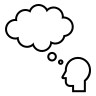
\includegraphics[width =\linewidth]{img/think1.png}
	\end{textblock*}
	
	\begin{textblock*}{2cm}(8cm,2cm)
		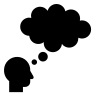
\includegraphics[width =\linewidth]{img/think2.png}
	\end{textblock*}
	
	Job recruitment, clinical assessment
\end{frame}

\begin{frame}{An example}
	\centering
	\begin{tikzpicture}
		\imagenode[0.5]{img/completeExample.png}
		
		
		
		
		\highlightbox[red,very thick]{0.12}{0.49}{0.85}{0.98}{red}{}{2}
		\highlightbox[green,very thick]{0.05}{0.01}{0.95}{0.45}{red}{}{3}
	\end{tikzpicture}
	
\end{frame}


\begin{frame}{An example: The matrix}
	\centering
	\begin{tikzpicture}
		\imagenode[0.5]{img/matrix.png}
		
		
		\highlighttext{0.2}{0.9}{0.8}{1}{red}{Change shapes \& numeric progression}{2}
		\highlightbox[red,very thick]{0.18}{0.65}{0.85}{0.9}{red}{}{2}
		\highlightbox[red,very thick]{0.18}{0.1}{0.38}{0.9}{red}{}{3}
		\highlighttext{0.1}{0.9}{0.4}{1}{red}{Numeric progression}{3}
	\end{tikzpicture}
\end{frame}

\begin{frame}{An example: The response list}
	

	\begin{textblock*}{3cm}(9cm,0.5cm)
	\includegraphics[width =\linewidth]{img/matrix.png}
\end{textblock*}


\begin{tikzpicture}
	\imagenode[0.4]{img/responses.png}
	

	\highlightbox[myGreen,very thick]{0.52}{0.05}{0.69}{.35}{circle,myGreen}{}{2-}
	\highlightbox[repetition,very thick]{0.52}{0.55}{0.69}{.82}{circle,myGreen}{}{3-}
	\highlightbox[repetition,very thick]{0.8}{0.05}{0.95}{.35}{circle,myGreen}{}{3-}
	\highlightbox[difference,very thick]{0.28}{0.55}{0.45}{.82}{circle,myGreen}{}{4-}
	\highlightbox[difference,very thick]{0.02}{0.05}{0.18}{.35}{circle,myGreen}{}{4-}
	\highlightbox[wp,very thick]{0.8}{0.55}{0.95}{.82}{circle,myGreen}{}{5-}
	\highlightbox[wp,very thick]{0.28}{0.05}{0.45}{.35}{circle,myGreen}{}{5-}
	\highlightbox[ic,very thick]{0.02}{0.55}{0.18}{.82}{circle,myGreen}{}{6-}
\end{tikzpicture}

\small 

\begin{table}
	
	\centering
	\begin{tabular}{p{3cm}p{8cm}}
		
		\onslide<3->\textcolor{repetition}{Repetition} & Repetition of a cell \textbf{adjacent} to the blank space \\
		\onslide<4->\textcolor{difference}{Difference} & Different in appearance from every element of the matrix\\
		\onslide<5->\textcolor{wp}{Wrong Principle} & Copy of a cell or combination of cells \\
		\onslide<6->\textcolor{ic}{Incomplete Correlate} & \textbf{Almost} the correct response \\
		
		
	\end{tabular}
	
\end{table}

\end{frame}

\section{Generating rules}

\begin{frame}
	
	\scalebox{.70}{
	\begin{tabular}{p{2cm}p{2.5cm} p{9cm}}
		\hline
		Category	&	Rule name	&	Definition	\\
		\hline
		Visuospatial rules	&	Object addition/subtraction	&	Visually merge two elements 	\\
		&	Movement	&	With a steady background, the movement is created by changing the position of an object across the cells	\\
		&	Rotation	&	The spatial orientation of the figure changes across the cells	\\
		&	Mental transformation	&	The third cell results from the application of the characteristics in the second cell to the figures in the first cell.	\\
		&	Numeric progression	&	Quantitative increase or decrease in the number of features from cell to cell	\\
		&	Changes in shape	&	The figures change across cells 	\\
		&	Changes in shade	&	The shading of the figures changes across cells 	\\
		&	Changes in size	&	The size of the figures changes across cells 	\\
		&	Changes in margins	&	The margins of the figures change across cells 	\\
		
		\hline
		Logical rules	&	AND	&	The third cell contains ONLY the elements that appeared in both the first and second cells 	\\
		&	OR	&	The third cell contains ALL the elements in the first and second cells	\\
		&	XOR	&	The third cell contains the elements in the first cell not present in the second cell and viceversa	\\
		\hline
	\end{tabular}}
\end{frame}

\section{The mat\texttt{R}iks package}


\begin{frame}{The mat\texttt{R}iks  architecture: Matriks generator}

	\begin{figure}
		\begin{tikzpicture}[node distance=1.5cm]
			\onslide<3->
			\node (start) [startstop] {Matrix generator};
			\onslide<1->
			\node (ob) [process, left of = start, yshift=1.5cm, xshift = -2cm] {Object};
			\onslide<2->
			\node (rule) [process, left of = start, yshift=-1.5cm, xshift = -2cm] {Rule};
			\onslide<4->
			\node (matrix) [rectangle ,right of = start, xshift = 3cm] {%
				\begin{tabular}{p{0.8cm} p{0.8cm} p{0.8cm}}
					Sq1 & Sq2 & Sq3  \\
					Sq4 & Sq5 & Sq6  \\
					Sq7 & Sq8 & Sq9  \\
			\end{tabular}};
			\onslide<3->	\path [->] (ob.east) edge (start.west);
			\onslide<3-> \path [->] (rule.east) edge (start.west);
			\onslide<4-> \path [->] (start.east) edge (matrix.west);
		\end{tikzpicture}
	\end{figure}
\end{frame}



\begin{frame}{}
	
	\begin{figure}
		\begin{tikzpicture}[node distance=1.5cm]
			\onslide<3->
			\node (start) [startstop] {\texttt{mat\_apply()}};
			\onslide<1->
			\node (ob) [process, left of = start, yshift=1.5cm, xshift = -2cm] {\includegraphics[width=\linewidth]{img/pacman.pdf}};
			\onslide<2->
			\node (rule) [process, left of = start, yshift=-1.5cm, xshift = -2cm] {\texttt{rotate}};
			\onslide<4->
			\node (matrix) [rectangle ,right of = start, xshift = 3cm] {\includegraphics[width=.40\linewidth]{img/pacmanMatrix.pdf}};
			\onslide<3->	\path [->] (ob.east) edge (start.west);
			\onslide<3-> \path [->] (rule.east) edge (start.west);
			\onslide<4-> \path [->] (start.east) edge (matrix.west);
		\end{tikzpicture}
	\end{figure}
\end{frame}

\begin{frame}{The mat\texttt{R}iks  architecture: Response options generator}
	
	\begin{figure}
		\begin{tikzpicture}[node distance=2cm]
			\onslide<2->
			\node (start) [startstop] {Response options generator};
			\onslide<1->
			\node (matrix) [rectangle ,above of = start] {%
				\begin{tabular}{p{0.8cm} p{0.8cm} p{0.8cm}}
					Sq1 & Sq2 & Sq3  \\
					Sq4 & Sq5 & Sq6  \\
					Sq7 & Sq8 & Sq9  \\
			\end{tabular}};
		\onslide<3->
					\node (response) [rectangle ,below of = start, yshift=-2.5] {%
			\scalebox{.70}{
				\centering
				\begin{tabular}{p{2.5cm} p{2.5cm}  p{2.5cm}p{2.5cm}}
				\multicolumn{4}{c}{correct}  \\
				IC-Flip & IC-Size & IC-Neg & IC-Inc\\
				R-Left & R-Diag & R-top & \\
				\multicolumn{2}{c}{WP-Copy} & \multicolumn{2}{c}{WP-Matrix} \\
				\multicolumn{4}{c}{Difference} 
				
			\end{tabular}
			}
		};
			\onslide<2-> \path [->] (matrix.south) edge (start.north);
			\onslide<3-> \path [->] (start.south) edge (response.north);
		\end{tikzpicture}
	\end{figure}
\end{frame}


\begin{frame}{}
	
	\begin{figure}
		\begin{tikzpicture}[node distance=2.5cm]
			\onslide<2->
			\node (start) [startstop] {\texttt{response\_list()}};
			\onslide<1->
			\node (matrix) [rectangle ,above of = start] {%
			\includegraphics[width=.40\linewidth]{img/pacmanMatrix.pdf}
				};
			\onslide<3->
			\node (response) [rectangle ,below of = start, yshift=-4] {%
			\includegraphics[width=.40\linewidth]{img/pacmanResponses.pdf}
			};
			\onslide<2-> \path [->] (matrix.south) edge (start.north);
			\onslide<3-> \path [->] (start.south) edge (response.north);
		\end{tikzpicture}
	\end{figure}
\end{frame}

\begin{frame}{(Some) of the available figures}
	\centering

		
			\begin{tabular}{c c c c}
			\includegraphics[width=0.2\linewidth]{img/pacman.pdf} & 
			\includegraphics[width=0.2\linewidth]{img/triangle.pdf} & 
			\includegraphics[width=0.2\linewidth]{img/malta.pdf} & 
			\includegraphics[width=0.2\linewidth]{img/maxi.pdf} \\
			\includegraphics[width=0.2\linewidth]{img/square.pdf} & 
			\includegraphics[width=0.2\linewidth]{img/lily.pdf} & 
			\includegraphics[width=0.2\linewidth]{img/hexagon.pdf} & 
			\includegraphics[width=0.2\linewidth]{img/luck.pdf} \\
			\includegraphics[width=0.2\linewidth]{img/bowtie.pdf} & 
			\includegraphics[width=0.2\linewidth]{img/ellipse.pdf} & 
			\includegraphics[width=0.2\linewidth]{img/ninja.pdf} & 
			\includegraphics[width=0.2\linewidth]{img/biscuit.pdf} \\
		\end{tabular}


\end{frame}


\begin{frame}{Visuospatial rules}
\begin{columns}[T]
	\begin{column}{.50\linewidth}
		\centering
		Rotate 
		
		\includegraphics[width=.7\linewidth]{img/rotate.pdf}
		
		Shade
		
		\includegraphics[width=.7\linewidth]{img/shade.pdf}
	\end{column}
	
	\begin{column}{.50\linewidth}
		\centering
		Shape 
		
		\includegraphics[width=.7\linewidth]{img/shape.pdf}
		
		Size
		
		\includegraphics[width=.7\linewidth]{img/size.pdf}
	\end{column}
\end{columns}
	
	\vspace{5mm}
	\centering
	\Large

$\ldots$
	
\end{frame}

\begin{frame}{Logical rules}
	\begin{columns}[T]
		\begin{column}{.50\linewidth}
			\centering
		AND ($\cap$)
		
		\includegraphics[width=.7\linewidth]{img/and.pdf}
		\end{column}
		
		\begin{column}{.50\linewidth}
			\centering
			OR ($\cup$)
			
				\includegraphics[width=.7\linewidth]{img/or.pdf}
		\end{column}
	\end{columns}
	
	\vspace{5mm}
	\centering
	
	XOR ($\Delta$)
	
		\includegraphics[width=.5\linewidth]{img/xor.pdf}
	
\end{frame}

\section{Why?}

\begin{frame}{PsycAssist}
	\begin{figure}
		\centering
		\includegraphics[width=.6\linewidth]{img/psyc.png}
	\end{figure}
	
	\pause
	
	\begin{exampleblock}{Sample}
		
		\footnotesize
		$n = 600$ children aged 4-11, recruited in Italian schools 
		
		$F = 48$\%
		
		$30$\% preschoolers
	
	\end{exampleblock}
	
	\pause
	
		\begin{exampleblock}{Stimuli}
		\footnotesize
		40 Raven-like matrices: 

		\begin{itemize}
			\item 5 Mono images 
			\item $2 \times 2$ matrices
			\item $3 \times 3$ matrices
		\end{itemize}
		
	\end{exampleblock}
\end{frame}

\begin{frame}{Rasch validation}
	
	\begin{itemize}
	\item Monotonicity check
	
	\item Fit the Rasch model: 
	
	\begin{enumerate}
		\item Item infit and outfit
		\item Local dependence
	\end{enumerate}
	\end{itemize}
	
	\pause
	
	\begin{block}{Note}
		
		2 matrices were eliminated because of technical issues 
		
		4 matrices were eliminated because a lack of monotonicity 
	
	\end{block}
	
	
\end{frame}

\begin{frame}{Starting model}

	
	The starting model included 34 matrices: 
	
	\begin{table}
		\centering
		\begin{tabular}[t]{c cc cc}
			\hline
			Madcov & SRMR & SRMSR & MADaQ3 & $p$-value\\
			\hline
			0.97 & 0.06 & 0.08 & 0.05 & $<0.001$\\
			\hline
		\end{tabular}
	\end{table}
	
	\vspace{10mm}
Oufit statistic suggested the underfit of one matrix (item 21) $\rightarrow$ removed and refitted the model 
	
	
	\begin{itemize}
		\item Check for infit/outfit $\rightarrow$ no matrices were identified as underfitting
		\item Check for local dependence: 
		
		\begin{itemize}
			\item Matrix $37 - 36$ $\rightarrow$ Matrix 37 eliminated
			\item Matrix $28 -  40$ $\rightarrow$ Matrix 40 eliminated
			
		\end{itemize}
	\end{itemize}
\end{frame}


\begin{frame}{The final model}

\begin{table}
	
	\centering
	\begin{tabular}[t]{ccccc}
		\hline
			Madcov & SRMR & SRMSR & MADaQ3 & $p$-value\\
		\hline
		0.96 & 0.06 & 0.08 & 0.05 & $<0.001$\\
		\hline
	\end{tabular}
\end{table}

\pause

\vspace{5mm}
\begin{figure}
\centering

\includegraphics[width=.7\linewidth]{img/icc.pdf}
\end{figure}
	
\end{frame}

\section{Final remarks}

\begin{frame}
	\begin{itemize}
		\item Generate similar but different matrices $\rightarrow$ parallel forms 
		
		\item Formalization of the matrix generation and response options generation processes
		
		\item Reproducibility of the stimuli
		
		\item Ease of use (for use\texttt{R})
		
		\pause
		\item[{\small\includegraphics[height=2.4ex]{img/soon.png}}] 
	\end{itemize}
	
\end{frame}

\begin{frame}
	
\end{frame}

\end{document}
